% 第 16 章：格点结果中的误差
% 译自：extract/sec16.txt（PDF 第 98-107 页），从 "16. Errors in Lattice
% Results" 标题到摘要末尾。摘要结束于句子中间
% ("...extrapolate keeping only the terms in")；第 16 节的结尾句和最后一段
% （位于 extract/sec17.txt 开头，PDF 第 108 页）根据作者原始来源
% （chap-errors.tex）补全，使本章完整。

\chapter{格点结果中的误差}

格点QCD的数值模拟会引入统计误差和一系列系统误差。我在此汇集了各种误差的简要描述，在本文其余部分我只给出定量估计。如果某一系统不确定度与某观测量在最先进计算中确定的统计误差相比在量级上可以忽略/相当，我将把它标记为可忽略/重要。

\section{统计误差}

用蒙特卡洛方法计算泛函积分采用的是统计抽样，因此结果具有统计误差。根据对用不同更新算法、不同初始组态和马尔可夫过程中不同随机数发生器产生的系综结果一致性的理解，目前认为淬火近似（QQCD）的泛函积分由单一区域主导。其次，我们发现，基于链变量小改变的马尔可夫链所产生的系综能够恰当地表示具有非平凡拓扑的组态。基于这些观测，我们得出结论：能量景观是简单的，因此统计误差应当按 $1/\sqrt{N}$ 下降，其中 $N$ 是独立测量的次数。用数据分组（binning）以及计算各种观测量的自关联时间等检验方法，来确定独立组态之间的蒙特卡洛时间。

对动力学模拟中去关联时间的估计刚刚开始出现，而对各种更新算法和不同费米子公式中去关联时间的理解也还不完整。最近一项利用混合蒙特卡洛算法 [141]（首选算法）研究威尔逊费米子更新的去关联的研究 [142] 给出了非常令人鼓舞的结果。他们发现，基于不同拓扑扇区之间隧穿率（预计属于最慢的模式之一）的去关联时间，与大威尔逊圈和强子关联函数等标准探针相差在两倍以内，并且在 $m_\pi / M_\rho \ge 0.56$ 时约为 $80$ 个分子动力学时间单位。因此，在当今计算机上可行的 5000--10000 单位的轨迹长度可以提供合理的统计样本。尽管像这种去关联时间如何随夸克质量减小而增长这样的细节仍需补充，但显然目前的蒙特卡洛算法确实为计算淬火QCD（QQCD）和完整QCD的泛函积分提供了可靠的方法。

\section{有限体积}

这是最容易直观理解的误差，因为它与用有限格点表示无穷系统有关。L\"uscher 已经证明，对于足够大的边长 $L$ 的格点，给定态质量 $M$ 的有限体积修正按 $e^{-ML}$ 衰减 [27]。这一分析假设与周期格点上的镜像态之间的相互作用很小。在小格点上，态的波函数被压缩，导致质量随格点尺寸减小而增长得更快。这一效应在 $L < 1.5$ 费米时清晰可见，此时有限尺寸行为符合幂律 $\sim 1/L^3$ [143]。因此，目标是在足够大的格点上工作，使有限尺寸效应被指数压低。

为了确定涉及夸克传播的观测量所需的格点尺寸，我选择$\pi$介子作为测试态，因为它最轻，因而具有最大的关联长度。淬火模拟的结果表明，对于 $M_\pi L \ge 5$，指数压低成立且修正可以忽略。对于物理值的 $M_\pi$，这相当于 $L \ge 7$ 费米。另一种表述这一判据的方式是：如果盒子尺寸大于 $7$ 费米，那么通常尺寸 $\le 1$ 费米的强子的量子力学性质就不会改变。目前的模拟探索的夸克质量范围为 $m_q \ge m_s/4$，等价地即 $M_\pi / M_\rho \ge 0.4$。对于这些「较重质量」，判据 $M_\pi L \ge 5$ 相当于 $L \ge 3$ 费米。最近的计算中所用的格点，例如后文将要讨论的 CP-PACS 运行，满足这一条件。

有限 $L$ 的另一个后果是动量分辨率。例如，对于 $L = 32$ 和 $1/a = 2$ GeV，最低的非零动量及其间隔为 $2\pi/La = 393$ MeV。在研究介子和重子的色散关系，或计算研究半轻子和稀有衰变中的形状因子所需的矩阵元时，人们希望有更精细的分辨率。这只能通过增大 $L$ 或 $a$ 来实现。增大 $L$ 受限于计算机资源，而增大 $a$ 会增加离散化误差，这将在下节讨论。

\section{有限格距误差}

格点只是一个技术性的脚手架，物理结果是通过取 $a \to 0$ 极限获得的。在有限 $a$ 处，格点结果具有离散化误差，其大小取决于格点作用量和算符被改进的程度（见第 8、12 和 13 节）。如第 8 节所讨论的，我们采用两种策略来消除这些误差。首先，改进格点作用量和算符，使在固定 $a$ 处误差很小；其次，在多个 $a$ 值处重复模拟并外推到 $a = 0$。由于用来描述误差的函数形式通常只截断到 $a$ 的首项，外推带有相应的系统误差。为了把握这一不确定性，对三种不同公式（威尔逊、三叶草、交错）进行了外推，它们的首项修正不同（$O(a)$、$O(\alpha a) - O(a^2)$、$O(a^2)$）。在 $a = 0$ 极限下三个结果的差异是对残余不确定性的度量。我将在第 20 节（讨论夸克质量的计算）说明这一控制离散化误差的方法。

\section{轻夸克质量的手征外推}

物理的 $u$ 和 $d$ 夸克质量太轻，无法在目前的格点上模拟。对于 $1/a = 2$ GeV，实际的模拟需要 $L/a \gtrsim 70$ 以避免有限体积效应，即保持 $M_\pi L \ge 5$。目前最大的格点尺寸是淬火的 $L/a = 32$ 和非淬火的 $L/a = 24$。因此，为了得到涉及轻夸克的量的结果，人们通常用由手征微扰论导出但只截断到前几项的函数形式，在 $m_u = m_d$ 上从 $m_s/4 - 2m_s$ 的范围进行外推。由于手征外推的范围很大，定量给出高阶手征修正的大小非常重要。这需要在大量夸克质量值处有精确的数据。目前大多数拟合只保留最低阶项，因为数据质量不足以定量给出各种高阶修正，和/或不足以识别第 16.8 节讨论的淬火人为效应。关于当前数据在分辨这些高阶修正方面的状况，将在第 18 节讨论，那里给出了对 $SU(3)$ 味对称性破缺的分析，例如重子八重态和十重态等 $SU(3)$ 多重态内介子与重子之间的质量差。

目前的模拟还忽略了同位旋破缺效应和电磁贡献，因为它们在性质上是几个 MeV，小于目前的数值分辨率。同位旋对称质量定义为 $\bar{m} = (m_u + m_d)/2$。关于在强 $U(1)$ 场存在下同位旋破缺效应的探索性分析，见文献~[144]。

我预计，由于可供格点QCD使用的计算能力提高了 10--100 倍，我们对手征修正的理解将在未来两年内发生重大变化。要恰当地研究同位旋破缺效应，需要 $m_u$ 和 $m_d$ 接近物理值的动力学格点。这样的模拟仍需数年才能实现。

\section{重夸克的离散化}

重夸克（$c$ 和 $b$）的模拟除 $O(\Lambda_{QCD}a)$ 和 $O(pa)$ 之外，还有 $O(ma)$ 的大离散化误差。这是因为在 $2\ \mathrm{GeV} \le 1/a \le 5\ \mathrm{GeV}$ 时，以格点单位测量的夸克质量 $m_c a$ 和 $m_b a$ 为量级 $1$。数据表明，即使在 $m_c$ 的情况下，对于威尔逊和三叶草作用量，这些离散化误差也很大。（对于重夸克，交错费米子相对于威尔逊型离散化没有任何优势，因此不用来研究重夸克。）为解决这一问题，人们正在研究若干替代方法（见第 13 节）。其中包括非相对论QCD（NRQCD）公式 [108]、重夸克有效理论的格点版本 [145]、一种在 NRQCD 与三叶草离散化之间插值的狄拉克离散化变体 [113]，以及非微扰 $O(a)$ 改进的 SW-三叶草费米子 [104]。许多合作组正在检验这些公式，但要判断哪种方法能为重夸克模拟提供最佳解决方案还为时过早。

\section{格点与连续方案之间的匹配（重整化常数）}

实验数据是用某种连续重整化方案（如 $\overline{MS}$）来分析的，因此为了与唯象学建立联系，必须把格点正规化方案中的结果转换到连续方案。$\overline{MS}$ 与格点方案中重整化量之间的微扰关系，在几乎所有情况下都只精确到 1 圈。数据表明，$O(\alpha_s)$ 修正可能很大，约 $10 - 50\%$，取决于所涉及的观测量。然而，正如 Parisi [77] 以及 Lepage 和 Mackenzie [78] 所解释的，这些大修正主要来自格点人为效应，一旦识别出它们来自蝌蚪图，就可以被消除。Lepage--Mackenzie 为消除这些人为效应而重整格点微扰论的处方，已经显著降低了相关的不确定性。尽管如此，改进并不均匀，在许多情况下修正仍然很大，而且蝌蚪图改进（TI）1 圈微扰估计中的残余误差很难确定。提高匹配因子可靠性的最后一步是发展非微扰方法 [146--148]。在建立这些计算方面已经取得了重大进展，一旦完成，现有结果中由于使用 1 圈 $Z$ 因子带来的不确定性将被消除。关于使用微扰与非微扰 $Z$ 因子效果的说明见第 20.1 节。

\section{算符混合}

如第 3 节所述，格点QCD的一个主要应用是计算强子态之间有效弱哈密顿量中出现的算符的矩阵元。除了这些算符的整体归一化问题之外，算符一般还会与相同维数、更高维数和\textit{更低}维数的算符混合。在格点上，这种混合由量子修正和离散化误差引起。由于在有限 $a$ 处格点理论的对称性比连续理论的对称性小，例如威尔逊费米子中手征对称性的硬破缺，需要考虑的格点算符集合通常比连续理论中的更大。在与低维算符混合的情况下，混合系数必须非常精确地知道，否则幂次发散会在 $a \to 0$ 时淹没信号。类似地，在与相同维数但不同张量结构的算符混合的情况下（例如由于手征对称性的显式破缺，在威尔逊型作用量中就会出现这种情况），如果系数不精确已知，手征行为同样可能完全被这些格点人为效应淹没。这种混合带来严重计算挑战的例子有：计算 $\Delta I = 1/2$ 规则、$B_K$、$B_6$ 和 $B_8$ 所需的 4-费米子算符的矩阵元。在这些情况下，非微扰地计算混合系数也是必不可少的。有关这些方法的讨论，见 Martinelli 教授的讲义。

\section{淬火近似 (QQCD)}

这一近似在计算上最难摆脱，也最难定量化。由于它在当今的模拟中起着关键作用，我将较详细地讨论它。该近似包括忽略路径积分中的费米子贡献，即在式~4.3 中令 $\det M = \mathrm{constant}$。这一近似的唯一原因是计算机能力的限制。用已知算法，完整QCD模拟的计算需求会因夸克质量的不同而增加 $10^3 - 10^5$ 倍。由于 QQCD 是禁闭的、渐近自由的，并表现出自发手征对称性破缺（$\langle \bar{\psi}\psi\rangle_{QQCD} \neq 0$），且与完整QCD的差别仅在于背景规范组态的相对权重，因此在大多数情况下物理分析是相同的。因此，人们认为进行详细的淬火模拟以理解并控制所有其他误差来源是合理的，同时等待更好的算法或提供所需额外 $10^3 - 10^5$ 倍（即 10--1000 太拉浮点运算能力）的计算机技术。

\begin{figure}[htbp]
\centering
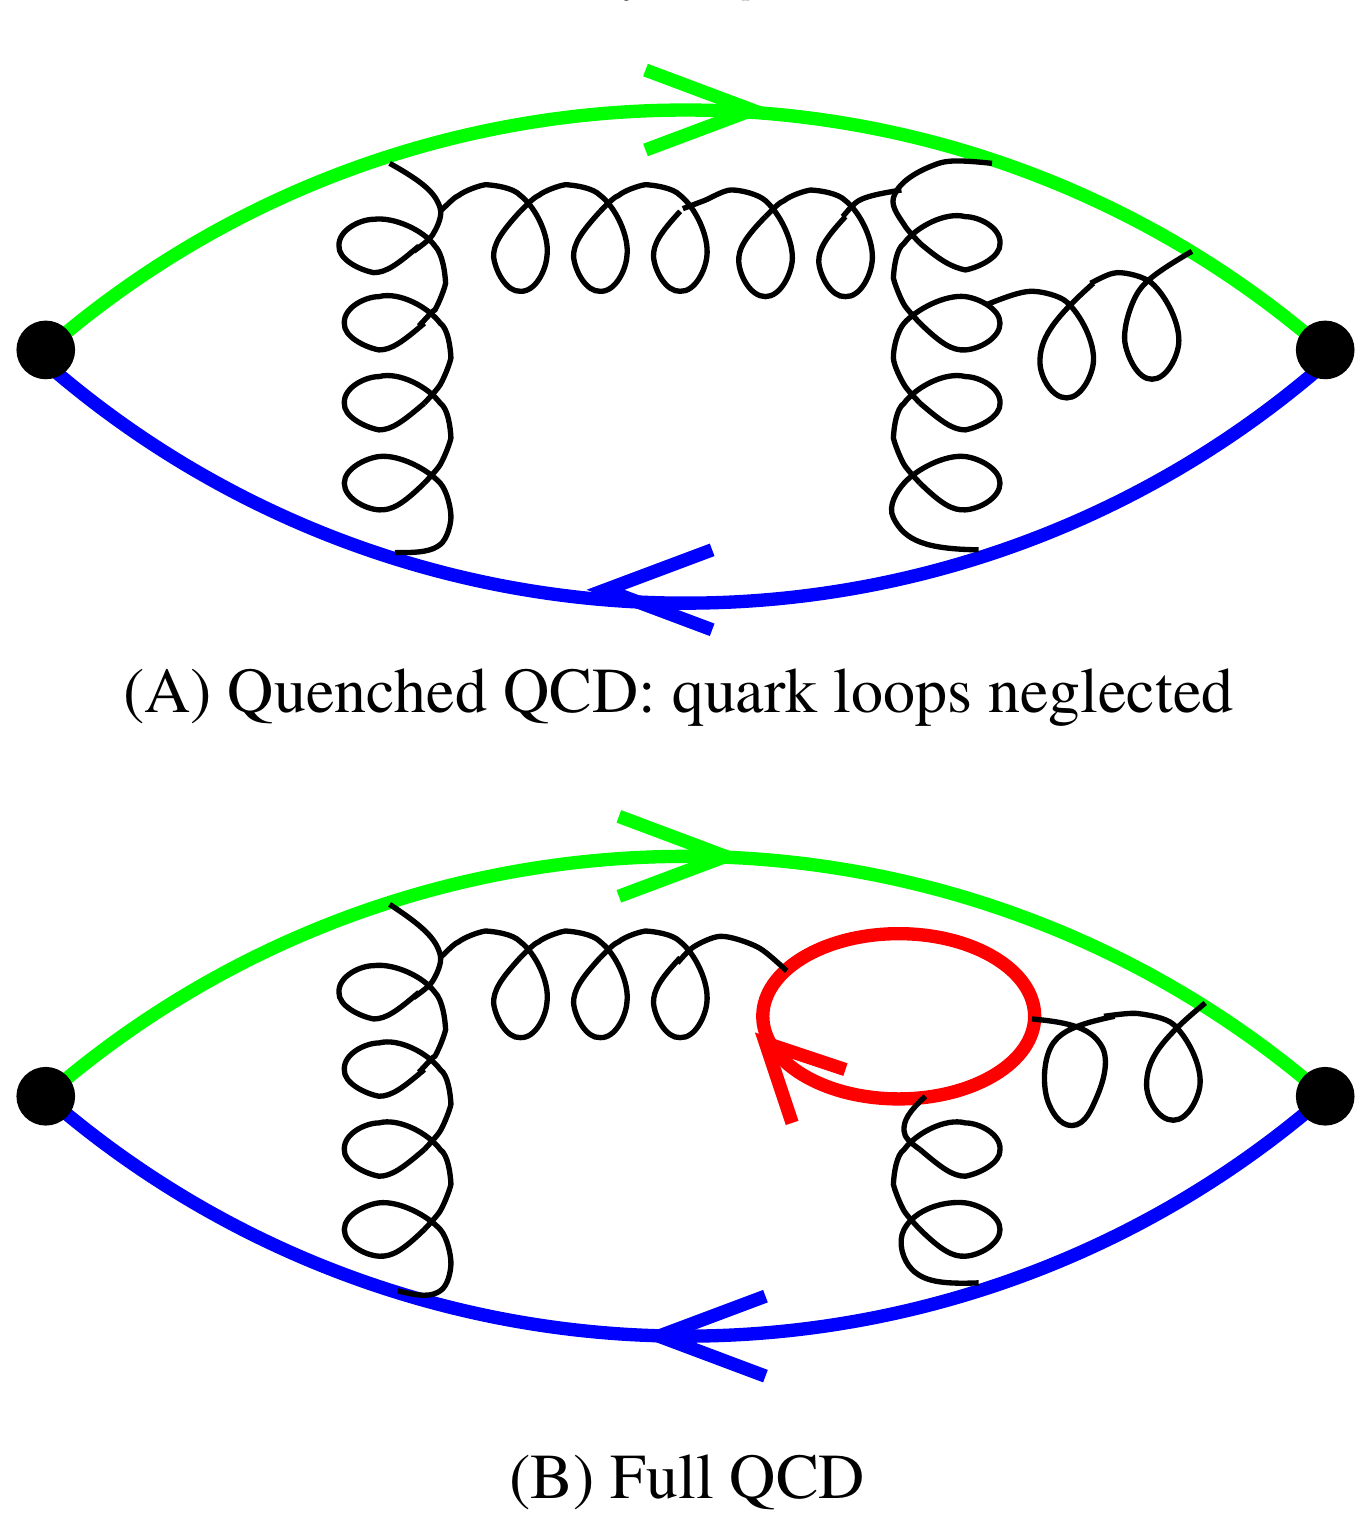
\includegraphics[width=0.8\textwidth]{images/fig16.png}
\caption{淬火QCD与QCD之间差异的示意图。QQCD 在虚胶子线上没有真空极化圈。}
\label{fig:16}
\end{figure}

从物理上说，淬火近似相当于关掉夸克圈的真空极化效应。这在图~\ref{fig:16} 中以$\pi$介子关联函数为例进行了说明。忽略真空极化效应的一个重要后果是 $q\bar{q}$ 对之间势能作为分离距离函数的行为。在完整理论中，弦通过从真空中产生 $q\bar{q}$ 对而断裂，因此在大距离处两个介子之间存在屏蔽势。对于这种屏蔽势，大威尔逊圈应显示周长律。在 QQCD 中，弦不会断裂，大威尔逊圈显示面积律。因此，这两种理论的长距离行为非常不同，人们可能会认为 QQCD 是一个糟糕的近似。然而，由于禁闭，与强子物理相关的长距离标度有一个几费米的自然截断。因此，如果能将某个精细标度（$\sim 0.01$ 费米，低于此标度渐近自由使计算成为微扰的）与强子的典型尺寸（$\sim 1$ 费米）之间的势能匹配起来，那么 QQCD 就能对强子谱给出合理的估计。这一论证实际上只适用于势模型工作良好的重夸克偶素。对于轻夸克，只能通过做模拟来估计畸变的大小。无论如何，学界已经通过假设这两种理论可以通过在某个标度（如 $0.5$ 费米）调整淬火耦合常数来大致匹配，等价地即调整整体标度 $\Lambda_{QQCD}$，并希望在许多情况下淬火修正很小，为 $10 - 20\%$，来推进工作。如果这一点得到证实，那么即使是 QQCD 也能产生许多对唯象学有用的预言。

尽管有这种乐观态度，但事实仍然是 QQCD 不是幺正理论，因此理解它如何失效很重要。我想用下面的例子来说明它的缺点。

我们可以通过测量图~\ref{fig:17}A 所示的三点函数 $\langle T[\rho\pi\pi]\rangle$ 来计算 QCD 和 QQCD 中的 $\rho\pi\pi$ 耦合。两个值之间的差异是衡量 QQCD 有效性的度量。另一方面，图~\ref{fig:17}B 所示的图在 QQCD 中不存在，$\rho$ 谱函数没有从 $2M_\pi$ 开始的割。因此，$\rho\pi\pi$ 耦合\textit{不能}从 QQCD 中 $\rho$ 两点函数的分析中提取出来。

\begin{figure}[htbp]
\centering
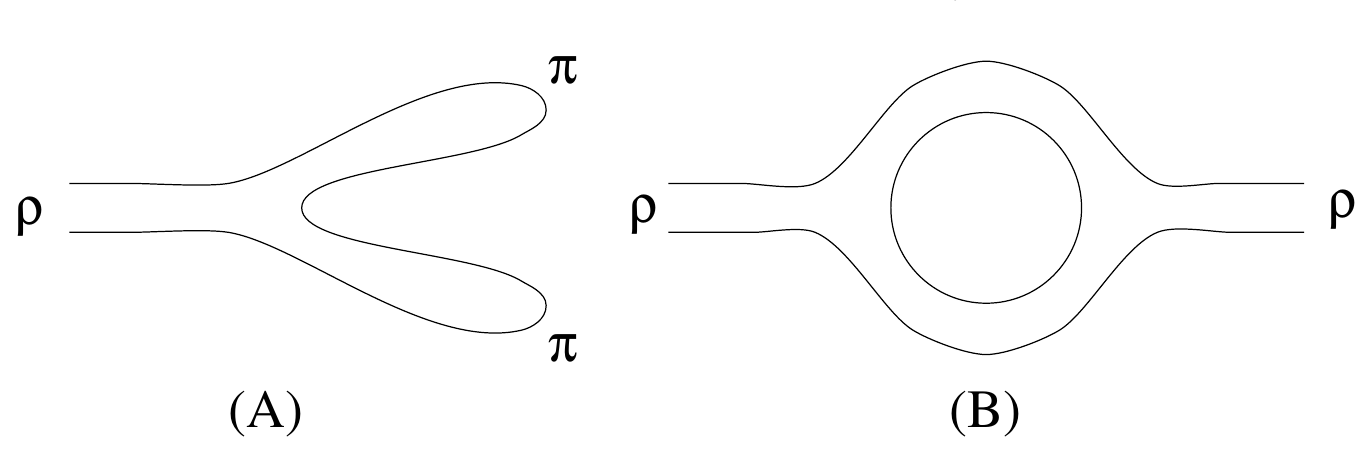
\includegraphics[width=0.8\textwidth]{images/fig17.png}
\caption{由 $\rho \to \pi\pi$ 衰变得到的 $\rho\pi\pi$ 耦合与 (B) 完整QCD 中的 $\rho$ 关联函数。}
\label{fig:17}
\end{figure}

完整QCD 与 QQCD 之间一个非常重要的差别是 $\eta'$ 的行为。在完整QCD 中，单态轴流是反常的，$\eta'$ 由于图~\ref{fig:18} 所示真空极化图的求和而获得很大的质量，
\begin{equation}
\frac{1}{p^2 - M^2} + \frac{1}{p^2 - M^2} M_0^2 \frac{1}{p^2 - M^2} + \cdots = \frac{1}{p^2 - M^2 - M_0^2}
\end{equation}
其中为简单起见，我把胶子耦合近似为一个与动量无关的常数 $M_0^2$。它通过 Witten--Veneziano 关系 $M_0^2 = 2n_f \chi_t / f_\pi^2 = M_{\eta'}^2 + M_\eta^2 - 2M_K^2$ [149] 与拓扑磁化率相联系。在 QQCD 中，真空极化图的缺失意味着 $\eta'$ 传播子具有单极点和双极点，即 $(p^2 - M^2)^{-1}$ 和「发夹」项 $(p^2 - M^2)^{-1} M_0^2 (p^2 - M^2)^{-1}$，其中 $M^2$ 是戈德斯通$\pi$介子质量 $M_\pi^2$。在 QQCD 的 $m_q \to 0$ 极限下 $\eta'$ 无质量这一事实具有重要的后果。两个小组，Sharpe 及其合作者 [150]，以及 Bernard 和 Golterman [151]，通过为 QQCD 构造一种把 $\eta'$ 保留为额外戈德斯通玻色子的手征微扰论研究了这些后果。我通过考虑$\pi$介子两点关联函数的行为来说明 $\chi$PT 与 Q$\chi$PT 之间的差异。

\begin{figure}[htbp]
\centering
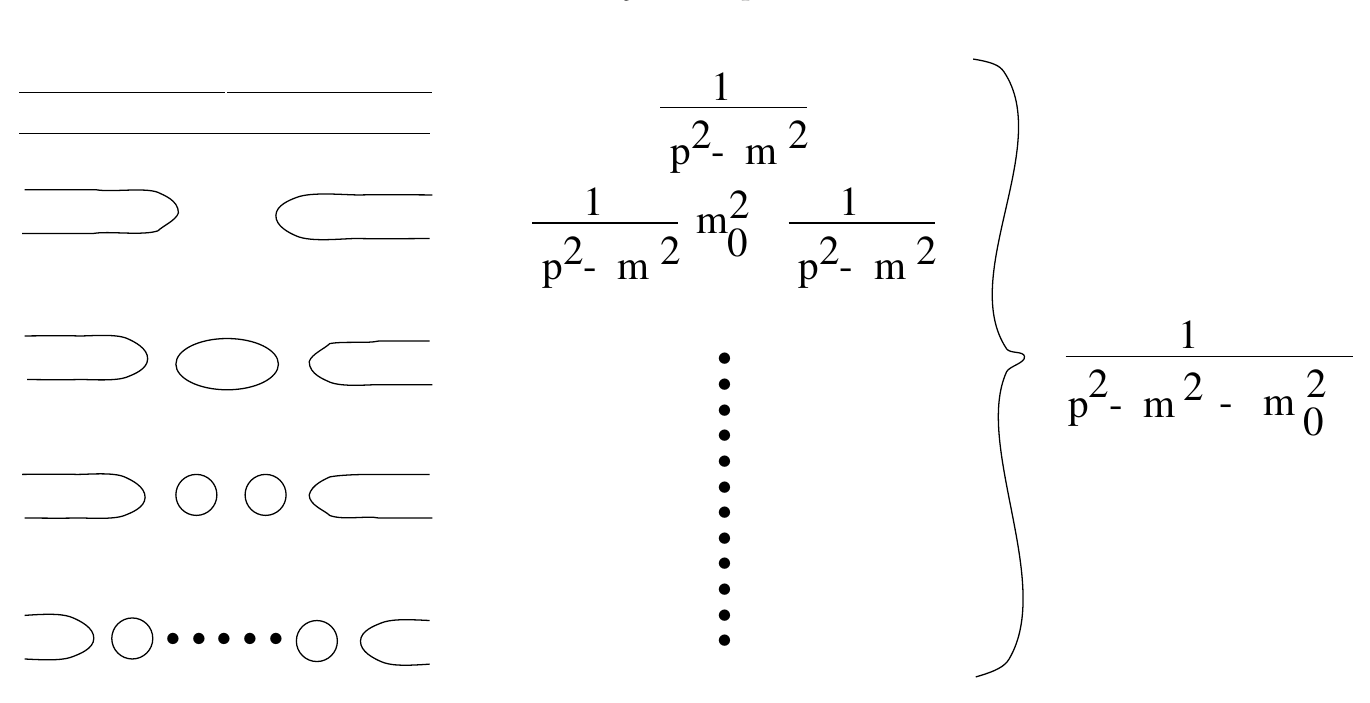
\includegraphics[width=0.8\textwidth]{images/fig18.png}
\caption{完整QCD 中 $\eta'$ 传播子的迭代。在 QQCD 中只有前两个图存活。}
\label{fig:18}
\end{figure}

\begin{figure}[htbp]
\centering
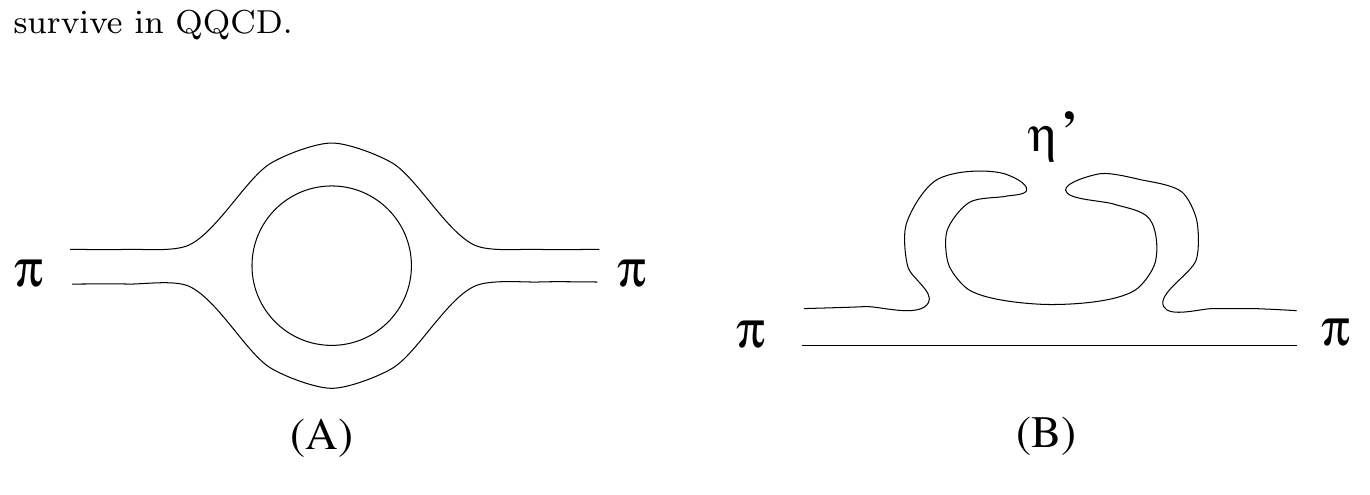
\includegraphics[width=0.8\textwidth]{images/fig19.png}
\caption{(A) 完整QCD (B) QQCD 中$\pi$介子传播子的 1 圈修正。}
\label{fig:19}
\end{figure}

在 1 圈阶，完整QCD 有图~\ref{fig:19}A 所示的图，而该图在 QQCD 中不存在。另一方面，在 QQCD 中，发夹项通过图~\ref{fig:19}B 所示的图给出贡献。这类图在完整QCD 中被忽略，因为它们迭代后会产生有质量的 $\eta'$。完整QCD 中 $M_\pi$ 和 $f_\pi$ 的手征展开已由 Gasser 和 Leutwyler 计算 [152]，
\begin{equation}
\begin{aligned}
M_\pi^2 &= 2mB\Bigl[1 + X_\pi - \frac{1}{3} X_{\eta_8} + \frac{16}{f_0^2}(2M_K^2 + M_\pi^2)(2L_6 - L_4) \\
&\qquad\qquad + \frac{16}{f_0^2} M_\pi^2 (2L_8 - L_5) + \cdots\Bigr] \\
f_\pi^2 &= f_0\Bigl[1 - 4X_\pi - 2X_K + \frac{16}{f_0^2}(2M_K^2 + M_\pi^2)L_4 + \frac{16}{f_0^2} M_\pi^2 L_5 + \cdots\Bigr]
\end{aligned}
\end{equation}
其中 $L_i$ 是 $O(p^4)$ 系数，$X_i = M_i^2 \log(M_i^2/\Lambda_{\chi SB}^2)/(4\pi f_0)^2$ 是手征对数，$f_\pi = 131$ MeV。在 QQCD 中，Sharpe 以及 Bernard 和 Golterman [150,151] 发现首项为
\begin{equation}
\begin{aligned}
M_\pi^{2Q} &= 2mB_Q\Bigl[1 - \delta \log\frac{M_\pi^2}{\Lambda_{\chi SB}^2} + \cdots\Bigr] \\
f_\pi^Q &= f_Q\Bigl[1 - \frac{16}{f_Q^2} M_\pi^2 \tilde{L}_5 + \cdots\Bigr]
\end{aligned}
\end{equation}
其中 $\delta = M_0^2 / 24\pi^2 f_\pi^2$，$\tilde{L}_i$ 是淬火的 $O(p^4)$ 系数。正比于 $\delta$ 的项是淬火手征对数，在 $m_q = 0$ 的极限下是奇异的。

一般说来，淬火与非淬火表达式之间的差异，正如上述表达式所示，为
\begin{itemize}
\item 两种理论中所有手征常数都不同。例如 $B \neq B_Q$ 和 $f_0 \neq f_Q$。
\item 正常的手征对数在 QQCD 中缺失。
\item 由于戈德斯通 $\eta'$，淬火表达式在手征极限下可以是奇异的，即通过正比于 $\delta$ 的项。随着 $m_q \to 0$，这些人为效应变得占主导地位。
\end{itemize}

Sharpe 以及 Bernard 和 Golterman 的分析提出的第一个问题是——淬火 $\chi$PT（一种关于 $m_q = 0$ 的展开）的结果，如果在该极限下是奇异的，它们还有意义吗？我们对此问题没有形式上的答案。采取的方法是做模拟，并通过做包含和不包含这些项的拟合来寻找这类手征对数。这一搜寻的现状已在 [153,154] 中综述。数据虽然不具有决定性，但确实表明 $\delta \approx 0.15$，与用 $M_0$ 和 $f_\pi$ 的唯象值得到的值一致。

第二个问题，假设淬火 $\chi$PT 的预言有意义，是对于需要外推到 $\bar{m}$ 的手征外推的量，如何提取对唯象学有用的结果？一种方法是在淬火人为效应很小的夸克质量区域内，用完整QCD手征展开拟合淬火数据。目前的数据表明这一区域是 $m_q \gtrsim m_s/4$。在这种情况下，淬火误差按定义是两类误差的组合：一类来自夸克圈的缺失，另一类来自在较重夸克质量处进行拟合。第二种可能做法是用 QQCD 表达式拟合，但外推时只保留完整QCD表达式中的项。这种方法缺点是增加了自由参数的数目。无论哪种情况，希望都是存在一些量，它们的 QQCD 人为效应很小，且 QQCD 与 QCD 系数之间的差异很小；在这种情况下，淬火估计就是有用的唯象预言。一个这样的例子是 $K^0\bar{K}^0$ 混合参数 $B_K$ [155]。

鉴于这些各种来源的系统误差，在格点上测量的任何量不仅依赖于输入参数，即夸克质量和耦合常数 $\alpha_s$，还依赖于格点尺寸 $L$、$a$（离散化误差 $\propto g^m a^n$，幂次取决于作用量和算符的改进阶数）、确定重整化常数的方法，以及动力学费米子味数 $n_f$。虽然对这些误差的理论理解一般还不完整，但已经知道很多，可以对数据做一致性检验。例如，固定 $n_f$ 模拟的无穷体积连续极限结果应当与离散化方案、所用的数值方法以及重整化常数的定义无关。截至撰写本文时，若干观测量的结果一旦外推到 $L \to \infty$ 和 $a \to 0$ 极限后显示出稳定性，尽管是在淬火近似（$n_f = 0$）下。我们把这视为朝着提供精确结果迈出的第一个重要步骤。我们的乐观源于知道，对许多唯象学上重要的量（$B_K$、$f_D$、$f_{D_s}$、$f_B$、$f_{B_s}$、$B_B$、$\alpha_s$ 和夸克质量），淬火格点QCD的结果已经能与最好的非格点方法相媲美，而未来方法论和计算机技术的改进将系统地提高它们的精度。
